\chapter{Molecuulorbitalen van tweeatomige moleculen}\label{ch:b2:diatomic-mos}

Giet vloeibare zuurstof tussen de polen van een sterke magneet en ze wordt
opzij getrokken; vloeibare stikstof valt er recht doorheen. Het zuurstofmolecuul draagt
ongepaarde elektronen, die door een magnetisch veld aangetrokken worden. Zijn lewisstructuur,
\ce{O=O} met alle elektronen gepaard, kan dat niet zeggen. \omterm{def:b2:diatomic-mos:lcao}{Molecuulorbitalen},
opgebouwd uit de atoomorbitalen van het vorige hoofdstuk, plaatsen elk elektron
van een molecuul in een eigen niveau: ze verklaren het magnetisme van
zuurstof, de sterkte en de lengte van bindingen, en de energieën die nodig zijn om
moleculen te ioniseren --- en ze leggen de grondslag voor de reactiviteit van de
hoofdstukken die volgen.

\begin{recall}
\Cref{ch:b2:atomic-orbitals}: atoomorbitalen, hun vormen, tekens en
energieën. Het deel van jaar~1: lewisstructuren, $\sigma$- en $\pi$-bindingen als
beschrijvende begrippen, hybridisatie en haar grenzen, ongepaarde elektronen en
radicalen.
\end{recall}

\begin{omfigure}
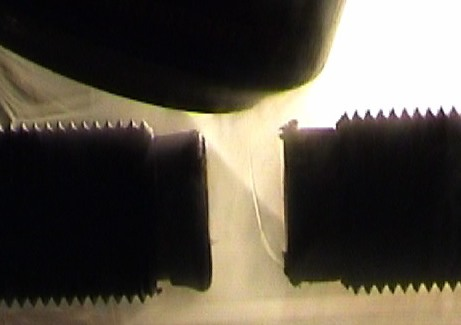
\includegraphics[width=0.42\linewidth]{images/book3/liquid-oxygen.jpg}

{\small Een dun straaltje vloeibare zuurstof dat tussen de polen van een sterke
magneet valt, wordt ernaartoe getrokken en hangt als een brug: het molecuul is
\omterm{def:b2:diatomic-mos:magnetism}{paramagnetisch}. (Foto: Pieter Kuiper, publiek domein, Wikimedia Commons.)}
\end{omfigure}

\section{De LCAO-methode}

\begin{definition}[Molecuulorbitaal]\label{def:b2:diatomic-mos:lcao}
Een \emph{molecuulorbitaal}\index{molecuulorbitaal} is de \omterm{def:b2:atomic-orbitals:wavefunction}{golffunctie} van één
elektron in een molecuul, uitgespreid over al zijn kernen. In de \emph{LCAO}\index{LCAO}-methode
(lineaire combinatie van atoomorbitalen) wordt ze geschreven als een som van
atoomorbitalen van de atomen, $\psi = \sum_i c_i\varphi_i$, met coëfficiënten die zo gekozen worden
dat de energie minimaal is.
\end{definition}

Voor twee atomen A en B, die elk één orbitaal inbrengen, is $\psi = c_A\varphi_A + c_B\varphi_B$.
De energie van een elektron in $\psi$, geminimaliseerd naar de coëfficiënten,
brengt drie getallen in het spel.

\begin{definition}[De integralen van de LCAO-methode]\label{def:b2:diatomic-mos:integrals}
Voor twee reële atoomorbitalen $\varphi_A$, $\varphi_B$ en de energieoperator $\hat H$
van een elektron in het molecuul:
\begin{itemize}
  \item de \emph{overlapintegraal}\index{overlapintegraal} $S = \int\varphi_A\varphi_B\,dV$
        meet in hoeverre de twee orbitalen hetzelfde gebied bezetten ($S = 1$ voor
        identieke, samenvallende orbitalen);
  \item de \emph{coulombintegraal}\index{coulombintegraal} $\alpha_A = \int\varphi_A\hat
        H\varphi_A\,dV$ is de energie van een elektron in $\varphi_A$ binnen het molecuul,
        dicht bij de atoomorbitaalenergie;
  \item de \emph{resonantie-integraal}\index{resonantie-integraal} $\beta = \int\varphi_A\hat
        H\varphi_B\,dV$, negatief, meet de koppeling van de twee orbitalen.
\end{itemize}
De energieën $E$ van de \omterm{def:b2:diatomic-mos:lcao}{molecuulorbitalen} zijn de wortels van de \emph{seculiere
determinant}\index{seculiere determinant}
\[
  \begin{vmatrix} \alpha_A - E & \beta - ES \\ \beta - ES & \alpha_B - E \end{vmatrix} = 0 .
\]
\end{definition}

De determinant komt uit het minimaliseren van $E = \int\psi\hat H\psi\,dV/\int\psi^2\,dV$
naar $c_A$ en $c_B$: de twee voorwaarden $\partial E/\partial c_A =
\partial E/\partial c_B = 0$ vormen een homogeen lineair stelsel, dat alleen een oplossing
verschillend van nul heeft wanneer zijn determinant nul is. Die variatiestap wordt hier
aangenomen.

\begin{theorem}[Twee identieke orbitalen]\label{thm:b2:diatomic-mos:homonuclear}
Voor $\alpha_A = \alpha_B = \alpha$ zijn de twee \omterm{def:b2:diatomic-mos:lcao}{molecuulorbitalen}
\[
  E_+ = \frac{\alpha + \beta}{1 + S}, \quad \psi_+ = \frac{\varphi_A + \varphi_B}{\sqrt{2(1 + S)}} ;
  \qquad
  E_- = \frac{\alpha - \beta}{1 - S}, \quad \psi_- = \frac{\varphi_A - \varphi_B}{\sqrt{2(1 - S)}} .
\]
\end{theorem}

\begin{proof}
De determinant geeft $(\alpha - E)^2 = (\beta - ES)^2$, dus $\alpha - E = \pm(\beta - ES)$.
Met het plusteken is $E(1 + S) = \alpha + \beta$; met het minteken $E(1 - S) = \alpha
- \beta$. Terug in het lineaire stelsel geeft $(\alpha - E)c_A + (\beta - ES)c_B = 0$ dat $c_B
= c_A$ voor $E_+$ en $c_B = -c_A$ voor $E_-$. Normering: $\int(\varphi_A \pm
\varphi_B)^2\,dV = 2 \pm 2S$.
\end{proof}

\begin{definition}[Bindende en antibindende orbitalen]\label{def:b2:diatomic-mos:bonding}
Een \emph{bindende orbitaal}\index{bindende orbitaal} ligt onder de atoomorbitalen waaruit ze
is opgebouwd: haar elektronendichtheid hoopt zich op tussen de kernen. Een
\emph{antibindende orbitaal}\index{antibindende orbitaal} ligt erboven en heeft een
\omterm{def:b2:atomic-orbitals:node}{knoopvlak} tussen de kernen. Een \emph{niet-bindende orbitaal}\index{niet-bindende orbitaal}
behoudt de energie van de atoomorbitaal, die geen partner vindt om
mee te combineren.
\end{definition}

\begin{proposition}[De antibindende orbitaal stijgt meer]\label{prop:b2:diatomic-mos:asymmetry}
Voor $S > 0$ wordt het antibindende niveau meer boven $\alpha$ opgetild dan het
bindende niveau eronder verlaagd wordt.
\end{proposition}

\begin{proof}
$E_+ - \alpha = (\beta - \alpha S)/(1 + S)$ en $E_- - \alpha = -(\beta - \alpha S)/(1 - S)$.
De teller $\beta - \alpha S$ is negatief (de koppeling overheerst), en $1 - S < 1
+ S$: de tweede verschuiving is in absolute waarde groter.
\end{proof}

Met twee elektronen, zoals in \ce{H2}, gaan beide in $\psi_+$ en is het molecuul stabieler
dan de afzonderlijke atomen. Met vier, zoals in \ce{He2}, moeten er twee in $\psi_-$,
wat meer kost dan $\psi_+$ oplevert: \ce{He2} is niet gebonden.

\begin{omfigure}
\begin{MOdiagram}[names, labels]
  \atom[H]{left}{ 1s = {0;up} }
  \atom[H]{right}{ 1s = {0;up} }
  \molecule[\ce{H2}]{ 1sMO = {.75;pair} }
\end{MOdiagram}
\hspace{1.5cm}
\begin{MOdiagram}[names, labels]
  \atom[He]{left}{ 1s = {0;pair} }
  \atom[He]{right}{ 1s = {0;pair} }
  \molecule[\ce{He2}]{ 1sMO = {.75;pair,pair} }
\end{MOdiagram}

{\small Molecuulorbitaaldiagrammen van \ce{H2} (\omterm{def:b2:diatomic-mos:bond-order}{bindingsorde} 1) en \ce{He2} (\omterm{def:b2:diatomic-mos:bond-order}{bindingsorde}
0, niet gebonden). Elk vakje is een niveau met hoogstens twee elektronen met
tegengestelde spin; gestreepte lijnen verbinden elke \omterm{def:b2:diatomic-mos:lcao}{molecuulorbitaal} met de atoomorbitalen
waaruit ze opgebouwd is.}
\end{omfigure}

\section{Overlap en symmetrie}

\begin{definition}[$\sigma$- en $\pi$-orbitalen]\label{def:b2:diatomic-mos:sigma-pi}
Een \emph{$\sigma$-orbitaal}\index{sigma-orbitaal@$\sigma$-orbitaal} van een lineair molecuul blijft onveranderd bij elke
rotatie om de molecuulas: ze heeft geen \omterm{def:b2:atomic-orbitals:node}{knoopvlak} dat de as bevat. Een
\emph{$\pi$-orbitaal}\index{pi-orbitaal@$\pi$-orbitaal} verandert van teken bij een rotatie over $180^\circ$ om de
as: ze heeft één \omterm{def:b2:atomic-orbitals:node}{knoopvlak} dat de as bevat. Een sterretje markeert \omterm{def:b2:diatomic-mos:bonding}{antibindende
orbitalen} ($\sigma^*$, $\pi^*$).
\end{definition}

\begin{proposition}[Overlap nul door symmetrie]\label{prop:b2:diatomic-mos:symmetry}
Twee orbitalen waarvan de ene symmetrisch en de andere antisymmetrisch is ten opzichte
van een vlak dat de molecuulas bevat, hebben overlap nul en \omterm{def:b2:diatomic-mos:integrals}{resonantie-integraal}
nul: ze combineren niet.
\end{proposition}

\begin{proof}
Spiegeling in het vlak laat de ruimte onveranderd maar keert het product
$\varphi_A\varphi_B$ om in het spiegelbeeldpunt: de bijdragen van de
twee helften van de ruimte aan $\int\varphi_A\varphi_B\,dV$ heffen elkaar op. Hetzelfde geldt voor
$\int\varphi_A\hat H\varphi_B\,dV$, omdat $\hat H$ de symmetrie van het molecuul heeft.
\end{proof}

Twee orbitalen wisselwerken sterk wanneer ze dezelfde symmetrie hebben (overlap verschillend
van nul), goed overlappen, en bij vergelijkbare energieën liggen. Een 1s-orbitaal van het ene atoom en een
$2\mathrm p_x$ van het andere ($x$ loodrecht op de as) combineren nooit;
$2\mathrm p_z$-orbitalen (langs de as) geven $\sigma$-orbitalen; $2\mathrm p_x$ en
$2\mathrm p_y$ geven twee paren $\pi$-orbitalen met gelijke energieën.

\begin{omfigure}
\begin{tikzpicture}[font=\small]
  % sigma 1s
  \pic at (0,0) {oms={0.85}}; \pic at (0.7,0) {oms={0.85}};
  \node at (0.35,-0.75) {$\sigma_{1s}$};
  \pic at (2.2,0) {oms={0.85}}; \pic at (2.9,0) {oms={-0.85}};
  \node at (2.55,-0.75) {$\sigma^*_{1s}$};
  % sigma 2p
  \pic at (4.6,0) {omp={-1}{0}}; \pic at (5.6,0) {omp={1}{0}};
  \node at (5.1,-0.75) {$\sigma_{2p}$};
  \pic at (7.4,0) {omp={-1}{0}}; \pic at (8.6,0) {omp={-1}{0}};
  \node at (8.0,-0.75) {$\sigma^*_{2p}$};
  % pi 2p
  \pic at (10.2,0) {omp={1}{90}}; \pic at (10.9,0) {omp={1}{90}};
  \node at (10.55,-0.95) {$\pi_{2p}$};
  \pic at (12.2,0) {omp={1}{90}}; \pic at (12.9,0) {omp={-1}{90}};
  \node at (12.55,-0.95) {$\pi^*_{2p}$};
  \draw[black!40, dashed] (-0.6,0) -- (13.4,0);
\end{tikzpicture}

{\small \omterm{def:b2:diatomic-mos:lcao}{Molecuulorbitalen} van een homonucleair tweeatomig molecuul, schematisch (de molecuulas
is horizontaal en gestreept). Combinaties in fase (bindend) verzamelen dezelfde
kleur tussen de kernen; combinaties in tegenfase (antibindend) plaatsen een
\omterm{def:b2:atomic-orbitals:node}{knoopvlak} ertussen. $\sigma$-orbitalen zijn symmetrisch rond de as; elke $\pi$-orbitaal
heeft de as in haar \omterm{def:b2:atomic-orbitals:node}{knoopvlak}.}
\end{omfigure}

\section{Homonucleaire tweeatomige moleculen van periode 2}

Met de 2s- en 2p-orbitalen van twee atomen van periode 2 ontstaan acht \omterm{def:b2:diatomic-mos:lcao}{molecuulorbitalen}:
$\sigma_{2s}$, $\sigma^*_{2s}$, $\sigma_{2p}$, twee $\pi_{2p}$, twee $\pi^*_{2p}$,
$\sigma^*_{2p}$.

\begin{proposition}[s-p-menging]\label{prop:b2:diatomic-mos:sp-mixing}
Voor \ce{O2} en \ce{F2} is de volgorde $\sigma_{2s} < \sigma^*_{2s} < \sigma_{2p} < \pi_{2p} <
\pi^*_{2p} < \sigma^*_{2p}$. Voor \ce{Li2} tot \ce{N2}, waarvan de 2s- en 2p-niveaus dicht bij elkaar liggen,
mengen de $\sigma$-orbitalen die uit 2s en $2\mathrm p_z$ gemaakt zijn: $\sigma_{2p}$ wordt omhooggeduwd tot boven
$\pi_{2p}$.
\end{proposition}

\begin{proof}[Redenering]
De orbitalen $\sigma_{2s}$ en $\sigma_{2p}$ hebben dezelfde symmetrie en kunnen met
elkaar combineren. Twee niveaus van dezelfde symmetrie stoten elkaar af (\cref{thm:b2:diatomic-mos:heteronuclear}
hieronder): $\sigma_{2s}$ daalt, $\sigma_{2p}$ stijgt, des te meer naarmate ze dicht bij elkaar liggen. De
afstand 2s--2p groeit langs de periode, dus het effect is groot aan de linkerkant en klein voor
zuurstof en fluor. De kruising tussen stikstof en zuurstof wordt aangenomen op grond van de
gemeten foto-elektronspectra.
\end{proof}

\begin{definition}[Bindingsorde]\label{def:b2:diatomic-mos:bond-order}
De \emph{bindingsorde}\index{bindingsorde} van een tweeatomig molecuul is $b = (n_b -
n_a)/2$, waarin $n_b$ en $n_a$ de aantallen elektronen in bindende en
\omterm{def:b2:diatomic-mos:bonding}{antibindende orbitalen} zijn.
\end{definition}

\begin{proposition}[Bindingsorde en binding]\label{prop:b2:diatomic-mos:bond-order}
Tussen atomen van hetzelfde paar elementen gaat een hogere \omterm{def:b2:diatomic-mos:bond-order}{bindingsorde} samen met een
kortere en sterkere binding; een \omterm{def:b2:diatomic-mos:bond-order}{bindingsorde} nul betekent geen binding.
\end{proposition}

\begin{proof}[Redenering]
Elk bindend elektron voegt dichtheid toe tussen de kernen en verlaagt de energie;
elk antibindend elektron neemt die weg en verhoogt de energie minstens evenveel
(\cref{prop:b2:diatomic-mos:asymmetry}). Het netto aantal bindende paren meet
de binding. De vergelijking is alleen zinvol voor vergelijkbare atomen: \ce{Li2} heeft
\omterm{def:b2:diatomic-mos:bond-order}{bindingsorde} 1 zoals \ce{F2}, maar zijn 2s-orbitalen zijn veel groter.
\end{proof}

\begin{definition}[Paramagnetisch en diamagnetisch]\label{def:b2:diatomic-mos:magnetism}
Een stof is \emph{paramagnetisch}\index{paramagnetisch} als haar moleculen
ongepaarde elektronen hebben: ze wordt in een magnetisch veld getrokken. Ze is
\emph{diamagnetisch}\index{diamagnetisch} als al haar elektronen gepaard zijn: ze wordt
zwak uit het veld geduwd.
\end{definition}

\begin{omfigure}
\begin{MOdiagram}[names, labels, style=square, distance=4.2cm, labels-fs=\scriptsize]
  \atom[N]{left}{ 2s = {0;pair}, 2p = {3.5;up,up,up} }
  \atom[N]{right}{ 2s = {0;pair}, 2p = {3.5;up,up,up} }
  \molecule[\ce{N2}]{ 2sMO = {.7;pair,pair}, 2pMO = {0.4/2.5,1.4;pair,pair,pair} }
\end{MOdiagram}
\hfill
\begin{MOdiagram}[names, labels, style=square, distance=4.2cm, labels-fs=\scriptsize]
  \atom[O]{left}{ 2s = {0;pair}, 2p = {3.5;pair,up,up} }
  \atom[O]{right}{ 2s = {0;pair}, 2p = {3.5;pair,up,up} }
  \molecule[\ce{O2}]{ 2sMO = {.7;pair,pair}, 2pMO = {1.8,.8;pair,pair,pair,up,up} }
\end{MOdiagram}

{\small Molecuulorbitaaldiagrammen van de valentieschil van \ce{N2} (links, met s-p-menging:
$\sigma_{2p}$ boven $\pi_{2p}$) en \ce{O2} (rechts). Stikstof: \omterm{def:b2:diatomic-mos:bond-order}{bindingsorde}
$(8 - 2)/2 = 3$, alle elektronen gepaard. Zuurstof: \omterm{def:b2:diatomic-mos:bond-order}{bindingsorde} $(8 - 4)/2 = 2$, met twee
ongepaarde elektronen in de twee $\pi^*$-orbitalen (regel van Hund): \ce{O2} is
\omterm{def:b2:diatomic-mos:magnetism}{paramagnetisch}. De diagrammen nemen $x$ als molecuulas, vandaar de labels
$2\sigma_x$, $2\pi_y$, $2\pi_z$.}
\end{omfigure}

\begin{method}[Een MO-diagram opbouwen en vullen]\label{met:b2:diatomic-mos:build-diagram}
\begin{enumerate}
  \item Plaats de valentie-atoomorbitalen van elk atoom op hun energie, het meest
        elektronegatieve atoom lager.
  \item Combineer orbitalen van dezelfde symmetrie: elk paar geeft één \omterm{def:b2:diatomic-mos:bonding}{bindende orbitaal}
        eronder en één \omterm{def:b2:diatomic-mos:bonding}{antibindende orbitaal} erboven; een orbitaal zonder partner blijft
        niet-bindend.
  \item Gebruik voor homonucleaire moleculen van periode 2 de volgorde met $\sigma_{2p}$ boven
        $\pi_{2p}$ tot en met stikstof, en eronder vanaf zuurstof.
\end{enumerate}
\end{method}

\begin{method}[Een gevuld diagram lezen]\label{met:b2:diatomic-mos:fill}
\begin{enumerate}
  \item Tel de valentie-elektronen (tel er één bij voor elke negatieve lading, trek er één af
        voor elke positieve lading).
  \item Vul van onderen, twee per orbitaal, met de regel van Hund voor ontaarde
        niveaus.
  \item \omterm{def:b2:diatomic-mos:bond-order}{Bindingsorde} $(n_b - n_a)/2$; ongepaarde elektronen geven paramagnetisme.
  \item Het hoogste bezette niveau wordt het eerst geïoniseerd.
\end{enumerate}
\end{method}

\begin{omfigure}
\small
\renewcommand{\arraystretch}{1.15}
\begin{tabular}{lcccccc}
 & \ce{Li2} & \ce{C2} & \ce{N2} & \ce{O2} & \ce{F2} & \ce{NO} \\ \hline
valentie-elektronen & 2 & 8 & 10 & 12 & 14 & 11 \\
\omterm{def:b2:diatomic-mos:bond-order}{bindingsorde} & 1 & 2 & 3 & 2 & 1 & 2.5 \\
ongepaarde elektronen & 0 & 0 & 0 & 2 & 0 & 1 \\
bindingslengte $r_e$ (pm) & 267.3 & 124.3 & 109.8 & 120.8 & 141.2 & 115.1 \\
$D_0$ (\unit{eV}) & 1.04 & 6.15 & 9.76 & 5.12 & 1.60 & 6.51 \\
\end{tabular}

\smallskip
{\small Tweeatomige moleculen van periode 2: \omterm{def:b2:diatomic-mos:bond-order}{bindingsordes} uit de MO-diagrammen; bindingslengten uit
spectroscopie, dissociatie-energieën $D_0$ uit getabelleerde vormingsenthalpieën
bij \qty{0}{K}, $D_0 = \Delta_f H_0(\mathrm A) + \Delta_f H_0(\mathrm B) - \Delta_f
H_0(\mathrm{AB})$.}
% ledger: re:Li2, re:C2, re:N2, re:O2, re:F2, re:NO, janafH0:Li, janafH0:Li2, janafH0:C, janafH0:C2, janafH0:N, janafH0:O, janafH0:F, janafH0:NO
\end{omfigure}

\section{Heteronucleaire tweeatomige moleculen}

\begin{theorem}[Twee orbitalen met verschillende energie]\label{thm:b2:diatomic-mos:heteronuclear}
Voor $\alpha_A > \alpha_B$ (B elektronegatiever), met $S$ verwaarloosd, $\bar\alpha = (\alpha_A
+ \alpha_B)/2$ en $\Delta = \alpha_A - \alpha_B$ geldt
\[
  E_\mp = \bar\alpha \mp \sqrt{\Delta^2/4 + \beta^2} .
\]
De \omterm{def:b2:diatomic-mos:bonding}{bindende orbitaal} (de lagere) heeft haar grootste coëfficiënt op B, de \omterm{def:b2:diatomic-mos:bonding}{antibindende
orbitaal} op A; wanneer $\Delta \gg |\beta|$, is $E_- \approx \alpha_B - \beta^2/\Delta$ en $E_+
\approx \alpha_A + \beta^2/\Delta$.
\end{theorem}

\begin{proof}
Met $S = 0$ zijn de energieën de eigenwaarden van $\begin{pmatrix}\alpha_A & \beta \\
\beta & \alpha_B\end{pmatrix}$: $(\alpha_A - E)(\alpha_B - E) = \beta^2$, waarvan de wortels
$\bar\alpha \pm \sqrt{\Delta^2/4 + \beta^2}$ zijn. Voor de lagere wortel is $(\alpha_B - E_-)c_B = -\beta
c_A$; $\alpha_B - E_- = \sqrt{\Delta^2/4 + \beta^2} - \Delta/2$ is kleiner dan $|\beta|$, dus
$|c_A| < |c_B|$. Voor $\Delta \gg |\beta|$ is $\sqrt{\Delta^2/4 + \beta^2} \approx \Delta/2 +
\beta^2/\Delta$.
\end{proof}

\begin{omfigure}
\begin{tikzpicture}
\begin{axis}[width=0.55\linewidth, height=6cm, xmin=0, xmax=8, ymin=-5, ymax=5,
  axis x line=bottom, axis y line=left, xlabel={$\Delta/|\beta|$}, ylabel={$E/|\beta|$},
  tick label style={font=\small}, label style={font=\small}]
\addplot[omThm, thick] table[x=d, y=Ehigh] {figdata/out/bachelor-2-two-level-a.dat};
\addplot[omDef, thick] table[x=d, y=Elow] {figdata/out/bachelor-2-two-level-a.dat};
\addplot[black!50, densely dotted] table[x=d, y=aA] {figdata/out/bachelor-2-two-level-a.dat};
\addplot[black!50, densely dotted] table[x=d, y=aB] {figdata/out/bachelor-2-two-level-a.dat};
\addplot[omThm, dashed] table[x=d, y=Phigh] {figdata/out/bachelor-2-two-level-a-pert.dat};
\addplot[omDef, dashed] table[x=d, y=Plow] {figdata/out/bachelor-2-two-level-a-pert.dat};
\node[font=\scriptsize, black!60, anchor=north west] at (axis cs:5.5,2.6) {$\alpha_A$};
\node[font=\scriptsize, black!60, anchor=south west] at (axis cs:5.5,-2.6) {$\alpha_B$};
\node[font=\scriptsize, omThm, anchor=south east] at (axis cs:3.2,2.2) {antibindend};
\node[font=\scriptsize, omDef, anchor=north east] at (axis cs:3.2,-2.2) {bindend};
\end{axis}
\end{tikzpicture}

{\small Twee wisselwerkende niveaus. Naarmate de afstand $\Delta$ tussen de atoomorbitalen groeit,
naderen de moleculaire niveaus (getrokken) de atomaire (gestippeld): de stabilisatie
$\beta^2/\Delta$ van de storingslimiet (gestreept) wordt klein. Bij $\Delta = 0$ is de
splitsing $2|\beta|$.}
\end{omfigure}

In waterstoffluoride ontmoet de 1s-orbitaal van waterstof de veel lagere 2p-orbitalen
van fluor. Alleen $2\mathrm p_z$, langs de as, heeft de juiste symmetrie: ze vormt
een bindende $\sigma$-orbitaal met het zwaartepunt op fluor, en een $\sigma^*$ met het zwaartepunt op
waterstof. De orbitalen $2\mathrm p_x$ en $2\mathrm p_y$ van fluor blijven
niet-bindend: het zijn zijn vrije elektronenparen. De binding is gepolariseerd naar fluor.

Koolstofmonoxide heeft de tien valentie-elektronen van \ce{N2} en een vergelijkbaar diagram,
maar de orbitalen van zuurstof liggen lager. Zijn \omterm{def:b2:diatomic-mos:bonding}{bindende orbitalen} liggen zwaarder op zuurstof;
zijn hoogste bezette orbitaal, een $\sigma$-orbitaal die zwaarder op koolstof ligt, is een vrij elektronenpaar
op koolstof. Koolstofmonoxide bindt metalen dus via koolstof
(\cref{ch:b2:coordination-complexes}).

\begin{omfigure}
\begin{tikzpicture}[font=\small]
  % CO schematic: C left (higher), O right (lower)
  \pic (c2s) at (0,0.6) {omlevel={ud}{0.8}}; \node[left] at (-0.5,0.6) {2s};
  \pic (c2p1) at (-0.45,2.6) {omlevel={u}{0.4}}; \pic (c2p2) at (0,2.6) {omlevel={u}{0.4}}; \pic (c2p3) at (0.45,2.6) {omlevel={empty}{0.4}};
  \node[left] at (-0.75,2.6) {2p};
  \node at (0,-0.6) {C};
  \pic (o2s) at (6,-1.2) {omlevel={ud}{0.8}}; \node[right] at (6.5,-1.2) {2s};
  \pic (o2p1) at (5.55,1.4) {omlevel={ud}{0.4}}; \pic (o2p2) at (6,1.4) {omlevel={u}{0.4}}; \pic (o2p3) at (6.45,1.4) {omlevel={u}{0.4}};
  \node[right] at (6.75,1.4) {2p};
  \node at (6,-2.2) {O};
  % MOs
  \pic (m1) at (3,-1.8) {omlevel={ud}{0.8}};
  \pic (m2) at (3,-0.2) {omlevel={ud}{0.8}};
  \pic (m3a) at (2.75,0.9) {omlevel={ud}{0.45}}; \pic (m3b) at (3.25,0.9) {omlevel={ud}{0.45}};
  \pic (m4) at (3,1.9) {omlevel={ud}{0.8}};
  \pic (m5a) at (2.75,3.3) {omlevel={empty}{0.45}}; \pic (m5b) at (3.25,3.3) {omlevel={empty}{0.45}};
  \pic (m6) at (3,4.4) {omlevel={empty}{0.8}};
  \draw[omcorr, densely dashed] (c2s-r) -- (m1-l) (o2s-l) -- (m1-r);
  \draw[omcorr, densely dashed] (c2s-r) -- (m2-l) (o2s-l) -- (m2-r);
  \draw[omcorr, densely dashed] (c2p3-r) -- (m3a-l) (o2p1-l) -- (m3b-r);
  \draw[omcorr, densely dashed] (c2p3-r) -- (m4-l) (o2p1-l) -- (m4-r);
  \draw[omcorr, densely dashed] (c2p3-r) -- (m5a-l) (o2p1-l) -- (m5b-r);
  \draw[omcorr, densely dashed] (c2p3-r) -- (m6-l) (o2p1-l) -- (m6-r);
  \node[omsymlabel, below=0.17cm, inner sep=0.5pt] at (m1-c) {$\sigma$};
  \node[omsymlabel, below=0.17cm, inner sep=0.5pt] at (m2-c) {$\sigma$};
  \node[omsymlabel, below=0.17cm, inner sep=0.5pt] at (3,0.9) {$\pi$};
  \node[omsymlabel, below=0.24cm, inner sep=0.5pt] at (m4-c) {$\sigma$ (vrij paar van C)};
  \node[omsymlabel, below=0.05cm, inner sep=0.5pt] at (3,3.3) {$\pi^*$};
  \node[omsymlabel, below=0.05cm, inner sep=0.5pt] at (m6-c) {$\sigma^*$};
  \node at (3,-2.6) {CO};
\end{tikzpicture}

{\small Valentieorbitalen van koolstofmonoxide, schematisch: de orbitalen van zuurstof liggen
lager dan die van koolstof. \omterm{def:b2:diatomic-mos:bond-order}{Bindingsorde} 3 zoals in \ce{N2}; de hoogste bezette
orbitaal is een $\sigma$-orbitaal die zwaarder op koolstof ligt: zijn vrij elektronenpaar.}
\end{omfigure}

\begin{history}[Hund en Mulliken]
\begin{minipage}[t]{0.27\linewidth}
\vspace{0pt}
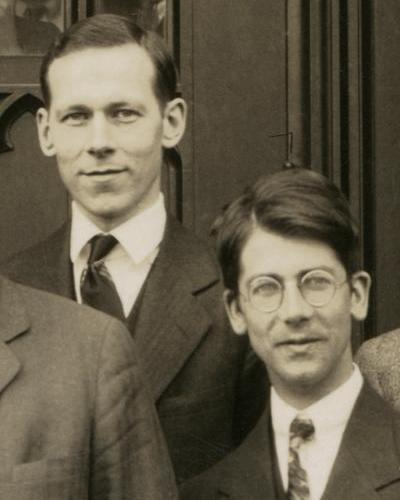
\includegraphics[width=\linewidth]{images/book3/mulliken-hund.jpg}
\end{minipage}\hfill
\begin{minipage}[t]{0.69\linewidth}
\vspace{0pt}
Tussen 1926 en 1932 interpreteerden Friedrich Hund en Robert Mulliken de spectra
van tweeatomige moleculen door elk elektron toe te wijzen aan een orbitaal van het hele
molecuul, ingedeeld naar zijn symmetrie rond de as. De woorden $\sigma$, $\pi$,
bindend en antibindend, en de orbitaaldiagrammen van dit hoofdstuk komen uit hun
werk; Mulliken kreeg in 1966 de Nobelprijs voor Scheikunde. De foto toont
Mulliken (links) en Hund in Chicago in 1929. (Foto: GFHund, CC BY 3.0,
Wikimedia Commons.)
\end{minipage}
\end{history}

\section{Ionisatie en bindingssterkte}

Een elektron uit een \omterm{def:b2:diatomic-mos:bonding}{bindende orbitaal} verwijderen verzwakt de binding; het uit
een \omterm{def:b2:diatomic-mos:bonding}{antibindende orbitaal} verwijderen versterkt haar. De dissociatie-energieën van de ionen
volgen uit een thermochemisch kringproces: voor $\mathrm{AB}^+ \to \mathrm A + \mathrm B^+$ geldt
\[
  D_0(\mathrm{AB}^+) = D_0(\mathrm{AB}) + I(\mathrm B) - I(\mathrm{AB}) ,
\]
waarbij B het atoom met de laagste ionisatie-energie is.

\begin{example}[Ionen van stikstof en zuurstof]\label{ex:b2:diatomic-mos:ions}
\ce{N2} ($I = \qty{15.58}{eV}$) verliest een bindend elektron: $D_0(\ce{N2+}) = 9.76 + 14.53 -
15.58 = \qty{8.71}{eV}$, zwakker dan \ce{N2}. \ce{O2} ($I = \qty{12.07}{eV}$) verliest een
$\pi^*$-elektron: $D_0(\ce{O2+}) = 5.12 + 13.62 - 12.07 = \qty{6.66}{eV}$, sterker dan \ce{O2},
in overeenstemming met de \omterm{def:b2:diatomic-mos:bond-order}{bindingsordes} 2.5 en 2.5 tegenover 3 en 2.
% ledger: ie:N2, ie:N, ie:O2, ie:O, janafH0:N, janafH0:O
\end{example}

\section{Oefeningen}

\begin{exercise}[$\star$]\label{exo:b2:diatomic-mos:1}
Neem voor twee 1s-orbitalen van waterstof $\alpha = \qty{-13.6}{eV}$, $\beta = \qty{-9.0}{eV}$ en
$S = 0.60$ (gegevens voor de oefening). Bereken $E_+$ en $E_-$, en daarna de energie van de twee
elektronen van \ce{H2} vergeleken met twee afzonderlijke atomen.
\end{exercise}

\begin{exercise}[$\star$]\label{exo:b2:diatomic-mos:2}
Geef de \omterm{def:b2:diatomic-mos:bond-order}{bindingsordes} van \ce{He2}, \ce{He2+}, \ce{Li2} en \ce{B2} (met s-p-menging).
\end{exercise}

\begin{exercise}[$\star$]\label{exo:b2:diatomic-mos:3}
Welke van \ce{B2}, \ce{C2}, \ce{N2}, \ce{O2}, \ce{F2} zijn \omterm{def:b2:diatomic-mos:magnetism}{paramagnetisch}?
\end{exercise}

\begin{exercise}[$\star$]\label{exo:b2:diatomic-mos:4}
De molecuulas is $z$. Welke paren onder (1s, $2\mathrm p_z$), (1s,
$2\mathrm p_x$), ($2\mathrm p_x$, $2\mathrm p_x$), ($2\mathrm p_x$, $2\mathrm p_y$),
(2s, $2\mathrm p_z$) hebben een overlap verschillend van nul?
\end{exercise}

\begin{exercise}[$\star\star$]\label{exo:b2:diatomic-mos:5}
Voorspel of \ce{N2+} een langere of kortere binding heeft dan \ce{N2}, en controleer met
zijn dissociatie-energie die in het hoofdstuk berekend is.
\end{exercise}

\begin{exercise}[$\star\star$]\label{exo:b2:diatomic-mos:6}
Koolstofmonoxide en \ce{N2} zijn iso-elektronisch. Leg uit waarom de \omterm{def:b2:diatomic-mos:bonding}{bindende orbitalen} van
CO zwaarder op zuurstof liggen en waarom zijn hoogste bezette orbitaal een vrij elektronenpaar op
koolstof is.
\end{exercise}

\begin{exercise}[$\star\star$]\label{exo:b2:diatomic-mos:7}
Welke orbitalen van fluor wisselwerken in HF met de 1s van waterstof, en welke blijven
niet-bindend? Teken het diagram.
\end{exercise}

\begin{exercise}[$\star\star$]\label{exo:b2:diatomic-mos:8}
Bereken met $\alpha_A = \qty{-10}{eV}$, $\alpha_B = \qty{-14}{eV}$ en $\beta = \qty{-3.0}{eV}$
(gegevens voor de oefening, $S$ verwaarloosd) de twee energieën en het gewicht $c_B^2$ van
de \omterm{def:b2:diatomic-mos:bonding}{bindende orbitaal} op B.
\end{exercise}

\begin{exercise}[$\star\star$]\label{exo:b2:diatomic-mos:9}
Toon aan dat \ce{C2} met s-p-menging \omterm{def:b2:diatomic-mos:bond-order}{bindingsorde} 2 heeft, opgebouwd uit twee $\pi$-bindingen en geen
$\sigma_{2p}$-binding.
\end{exercise}

\begin{exercise}[$\star\star\star$]\label{exo:b2:diatomic-mos:10}
Geef de \omterm{def:b2:diatomic-mos:bond-order}{bindingsordes} van NO en \ce{NO+}. Bereken uit $D_0(\ce{NO}) = \qty{6.51}{eV}$, $I(\ce{NO}) =
\qty{9.26}{eV}$ en $I(\ce{O}) = \qty{13.62}{eV}$ de waarde $D_0(\ce{NO+})$ voor $\ce{NO+} \to
\ce{N} + \ce{O+}$, en becommentarieer.
\end{exercise}

\begin{exercise}[$\star\star\star$]\label{exo:b2:diatomic-mos:11}
Toon aan dat $E_+ + E_- = 2(\alpha - \beta S)/(1 - S^2)$, en dat dit groter is dan $2\alpha$ wanneer
$\beta < \alpha S < 0$. Leid daaruit af waarom twee gevulde orbitalen elkaar afstoten (destabilisatie
met vier elektronen).
\end{exercise}

\begin{exercise}[$\star\star\star$]\label{exo:b2:diatomic-mos:12}
Rangschik \ce{O2+}, \ce{O2}, \ce{O2-}, \ce{O2^2-} naar \omterm{def:b2:diatomic-mos:bond-order}{bindingsorde}, bindingslengte en
bindingssterkte. Welk ion komt voor in waterstofperoxide, en welk in de gele
verbinding \ce{KO2}?
\end{exercise}

\section{Probleem: zuurstof en zijn ionen}

\begin{problem}[{Weekendprobleem --- het molecuulorbitaaldiagram van dizuurstof,
de bindingsordes en het magnetisme van zijn ionen, ionisatie en de sterkte van de
binding, en de twee manieren om de $\pi^*$-elektronen te paren}]
\label{pb:b2:diatomic-mos:1}
Gegevens: $I(\ce{O}) = \qty{13.62}{eV}$, $I(\ce{O2}) = \qty{12.07}{eV}$, $I(\ce{N}) =
\qty{14.53}{eV}$, $I(\ce{N2}) = \qty{15.58}{eV}$; $\Delta_f H_0$ bij \qty{0}{K}
(\unit{kJ/mol}): \ce{O} 246.79, \ce{N} 470.82; $r_e$: \ce{O2} \qty{120.8}{pm}, \ce{N2}
\qty{109.8}{pm}; $1\ \unit{eV} = \qty{96.485}{kJ/mol}$.
% ledger: ie:O, ie:O2, ie:N, ie:N2, janafH0:O, janafH0:N, re:O2, re:N2

\medskip
\noindent\textbf{Deel I --- Dizuurstof.}
\begin{enumerate}
  \item Hoeveel valentie-elektronen heeft \ce{O2}?
  \item Teken zijn MO-diagram van de valentieschil (zonder s-p-menging) en vul het.
  \item Bereken zijn \omterm{def:b2:diatomic-mos:bond-order}{bindingsorde}.
  \item Hoeveel ongepaarde elektronen? Is \ce{O2} \omterm{def:b2:diatomic-mos:magnetism}{paramagnetisch}?
  \item Waarom schiet de lewisstructuur hier tekort?
  \item Bereken $D_0(\ce{O2})$ in \unit{eV}.
\end{enumerate}

\medskip
\noindent\textbf{Deel II --- De ionen.}
\begin{enumerate}[resume]
  \item Geef de configuratie en de \omterm{def:b2:diatomic-mos:bond-order}{bindingsorde} van \ce{O2+}.
  \item Hetzelfde voor het superoxide-ion \ce{O2-}.
  \item Hetzelfde voor het peroxide-ion \ce{O2^2-}.
  \item Geef het aantal ongepaarde elektronen van elk ion.
  \item Rangschik \ce{O2+}, \ce{O2}, \ce{O2-}, \ce{O2^2-} naar voorspelde bindingslengte.
  \item Welk ion heeft een enkelvoudige O--O-binding, zoals waterstofperoxide?
  \item Welke van de vier deeltjes zijn \omterm{def:b2:diatomic-mos:magnetism}{paramagnetisch}?
\end{enumerate}

\medskip
\noindent\textbf{Deel III --- Ionisatie.}
\begin{enumerate}[resume]
  \item Uit welke orbitaal vertrekt het elektron wanneer \ce{O2} geïoniseerd wordt?
  \item Waarom is $I(\ce{O2})$ lager dan $I(\ce{O})$?
  \item Toon aan dat $D_0(\ce{O2+}) = D_0(\ce{O2}) + I(\ce{O}) - I(\ce{O2})$ en bereken het.
  \item Vergelijk met $D_0(\ce{O2})$ en verklaar.
  \item Bereken op dezelfde manier $D_0(\ce{N2})$ en $D_0(\ce{N2+})$.
  \item Waarom is $I(\ce{N2})$ hoger dan $I(\ce{N})$?
  \item Vat samen: wanneer versterkt ionisatie een binding?
\end{enumerate}

\medskip
\noindent\textbf{Deel IV --- De $\pi^*$-elektronen.}
\begin{enumerate}[resume]
  \item In de grondtoestand bezetten de twee $\pi^*$-elektronen twee verschillende orbitalen met
        parallelle spins. Welke regel zegt dat?
  \item Beschrijf een toestand waarin beide dezelfde $\pi^*$-orbitaal bezetten.
  \item Waarom ligt die toestand hoger in energie?
  \item Wat zijn zijn \omterm{def:b2:diatomic-mos:bond-order}{bindingsorde} en zijn magnetisme?
  \item Geef de \omterm{def:b2:diatomic-mos:bond-order}{bindingsorde} van \ce{O2+} en zijn dissociatie-energie.
\end{enumerate}
\end{problem}
